\documentclass[a4paper,titlepage]{article}
\title{Zelflerende Systemen}
\author{Steven Bronsveld en Thijs van Loenhout}
\usepackage[dutch]{babel}
\usepackage{graphicx}
\usepackage{multirow}
\usepackage{blindtext}
\usepackage{csquotes}
\usepackage{float}
\usepackage{amsmath}
\usepackage[backend=bibtex,sorting=none]{biblatex}
\usepackage{color}
\definecolor{praktijk}{rgb}{1,0.5,0}



\usepackage[a4paper, total={8in, 12in}]{geometry}



\bibliography{references.bib}

\MakeOuterQuote{"}

\graphicspath{ {res/} }

\begin{document}

\begin{titlepage}

\maketitle
\end{titlepage}

\renewcommand{\contentsname}{Inhoud}

\newpage
\tableofcontents



\newpage
\section{Inleiding}
Elk jaar boekt de mens grootschalige vorderingen op het gebied van computers, zowel hardware als software. Iets waar wij echter nog niet in geslaagd zijn te maken, is een ware \textbf{ Artificial Intelligence}, al lukt het steeds beter een illusie van denken te cre\"eren. Voorbeelden zijn de persoonlijke assistenten die inmiddels in elke smartphone ge\"integreerd zijn. \textit{Siri}, \textit{Google Now} en \textit{Cortana} maken gebruik van spraakherkenning om de gebruiker de gevraagde informatie te tonen, maar denken zoals mensen doen ze hierbij niet. \\

Al lange tijd interesseerden wij ons in onderwerpen als "computers", "programmeren" en ook "AI", maar de laatste bracht nog erg veel vragen met zich mee. Het leek ons als een mysterieus verschijnsel dat een programma zichzelf kon verbeteren. Onze vragen bleven enige tijd onbeantwoord terwijl we met de alledaagse schooltaken bezig waren... En toen kwam het profielwerkstuk. We hadden lichte keuzestress over het onderwerp, maar terugkijkend was een AI-gerelateerd onderwerp niet te vermijden. We kregen de kans ons te verdiepen in dit mysterieuze onderwerp en grepen deze vol enthousiasme.

Boven alles wilde wij zelf iets leren van dit verslag en zelf met het onderwerp bezig zijn, en niet klakkeloos de informatie overnemen die een ander al op internet had geplaatst. Dit zou uiteindelijk betekenen dat we verschillende programma's hebben geschreven, ter illustratie bij de tekst, om zelf de stof beter te begrijpen of simpelweg omdat het leuk was ermee bezig te zijn. Ook hebben wij twee grote programma's, een voor \textit{Digit Recognition} en het spelen van een spel, geschreven die ons moeten helpen bij het beantwoorden van de vraag die wij ons hebben gesteld: \textit{In welke aspecten verschillen diverse zelflerende computersystemen, ontworpen voor \'e\'en specifieke taak, van elkaar?}

In het oriëntatieproces liepen wij vrij natuurlijk van de ene vraag op de andere. Het beantwoorden van al deze vragen hebben wij in de eerste 7 hoofdstukken beschreven in het theoriedeel van dit verslag. De kennis die wij hier hebben opgedaan, zouden we later gebruiken voor de twee grote programma's. Dit staat beschreven in de hoofdstukken 8 en 9.



\newpage

\section{Reguliere algoritmes}

\subsection{Inleiding}
Voordat we onderzoek kunnen doen naar zelflerende algoritmes moeten we eerst een beeld krijgen van niet-zelflerende algoritmes. Dit noemen we in dit verslag \textit{reguliere algoritmes}. We behandelen in dit hoofdstuk de vraag: \textit{Wat zijn voorbeelden van reguliere algoritmes en hoe werken ze?} We nemen twee bekende zoekalgoritmes als voorbeeld.


\subsection{Verschillende algoritmes}
Computers hebben geen bewustzijn. Om deze reden kunnen ze niet zelf bepalen iets te doen. Waar computers wel in uitblinken, is het uitvoeren van taken die hun zijn opgelegd. Deze taken in de vorm van code. Via code kun je computers opdrachten geven, bijvoorbeeld: \textit{Bereken 7 * 6}. De boodschap valt echter niet op deze manier over te brengen. Afhankelijk van de taal waarin je programmeert zijn er vaste commando's waar de computer op zal reageren.
Naarmate de opdracht die je een computer wil laten uitvoeren complexer wordt, zal ook het gebruik van deze commando's ingewikkelder worden. Hier komen algoritmes in het spel. Een algoritme is een soort stappenplan, waarin een complexere handeling in duidelijke opdrachten weergegeven wordt. De volgende definitie geeft een betekenis in de meest algemene zin: \textit{"een algoritme is een eindige reeks instructies om vanaf een beginpunt een bepaald doel te bereiken."} \cite{WoordenOrg}

Een toegankelijke vergelijking is koken. Er is een \textbf{input} van voedsel waar uiteindelijk een gerecht uit moet komen, de \textbf{output}. Voor het tot stand komen van dit gerecht gebruik je een recept. Dit recept is als het ware het algoritme.
Het aantal mogelijke algoritmes is enorm groot. Niet alleen is het een ruim begrip, ook kan het desbetreffende doel waarschijnlijk op meerdere manieren bereikt worden. Het ene algoritme zal misschien beter zijn dan het andere doordat het bijvoorbeeld effici\"enter werkt.

Uiteraard zijn er ook vele algoritmes die gebruik maken van toepassingen, zoals een \textbf{queue} en een \textbf{stack}, die betrekking hebben tot ons onderwerp. Enkele hiervan zullen hier beschreven worden.

\subsubsection{Breadth-first search (BFS)}
Dit algoritme, bedacht in de jaren vijftig van de vorige eeuw door E.F. Moore \cite{Moore}, een Amerikaans professor in de wiskunde en computer sciences en een voortrekker in kunstmatig leven, is een zoekalgoritme voor datasets in de vorm van grafieken of "boom"-structuren. In deze dataset, een (grote) verzameling data (zie figuur \ref{fig:datasetBFS3}), wordt \'e\'en \textbf{node}, een item uit de dataset, als oorsprong benoemd, de \textbf{root}. Ook wordt een bepaalde uitkomst als doel gesteld. Vervolgens krijgt elke node drie waardes aangewezen:
\begin{itemize}
\item De afstand van de huidige node naar de root. Dit is het aantal stappen dat gezet moet worden om bij de root te komen. 
\item De node die v\'{o}\'{o}r de huidige node kwam, de \textbf{predecessor}. Anders gezegd: bij welke node je uitkomt als je een enkele stap terug zet.
\item Een \textbf{state}. De state houdt bij of de node al gecontroleerd is.
\end{itemize}

Bij Breadth-first search wordt gebruik gemaakt van een queue. Dit is een lijst waar nodes aan toegevoegd en uitgehaald kunnen worden. Net zoals een daadwerkelijke wachtrij wordt het "\textit{eerste erin, als eerste eruit}" principe toegepast.
Het Breadth-first search algoritme ziet er als volgt uit:

\begin{enumerate}
\item Maak een lege lijst S voor bezochte nodes.
\item Maak een lege lijst Q met de queue.
\item Benoem \'e\'en node als root en voeg deze toe aan S.
\item Voeg de root toe aan Q. 
\item Zolang Q niet leeg is:
	\begin{enumerate}
	\item Haal de voorste node uit de queue. Dit is de \textit{current} node.
	\item Als current het doel is:
		\begin{enumerate}
		\item Return current.
		\end{enumerate}
	\item Voor elke node die grenst* aan current:
		\begin{enumerate}
		\item Als deze node nog niet bezocht is en dus niet in S zit:
			\begin{enumerate}
			\item Voeg de node toe aan S.
			\item Zeg dat de predecessor van de node de current node is.
			\item Haal de node uit de queue.
			\end{enumerate}
		\end{enumerate}
	\end{enumerate}
\end{enumerate}

\textit{*Aangrenzend zijn betekent hier \textit{in directe verbinding staan met}.}

\begin{figure}[h]
  \centering
    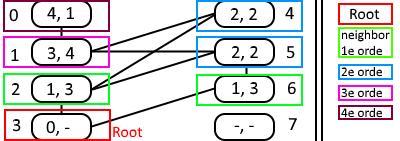
\includegraphics[width=\textwidth]{datasetBFS3.png}
  \caption{Schematische weergave van een willekeurige dataset, waarop het Breadth-first search algoritme wordt toegepast.}
  \label{fig:datasetBFS3}
\end{figure}
Hierboven is een voorbeeld van een simpele dataset weergegeven (zie figuur \ref{fig:datasetBFS3}), genummerd van node 0 tot en met node 6. Node 3 is de root en node 0 het doel. Om bij het doel te komen wordt het Breadth-first search algoritme toegepast. Node 3, de root, wordt toegevoegd aan de lijsten Q en S. Node 3 wordt weer uit de queue gehaald en \'e\'en voor \'e\'en worden de aangrenzende nodes bekeken. Hierbij worden ze toegevoegd aan de stack. Omdat zowel 2 als 6 het niet het doel zijn, herhaald het algoritme zich. Nu wordt 2 bekeken. Het doel is niet gevonden in de aangrenzende nodes. Daarna komt 6, ook zonder succes. (Let hierbij op dat node 5 niet nogmaals bekeken wordt, dit is namelijk al bij node 2 gedaan en is dus al aanwezig in lijst S). Intussen zijn node 4 en node 5 toegevoegd aan de queue, ze zijn immers verbonden met node 2. Ook hier wordt het proces herhaald, node 1 zit nu in de queue. Uiteindelijk wordt node 1 bekeken en wordt het doel, node 0, gevonden.

Met BFS kan je zo de weg van de root naar het doel achterhalen. Dit is nuttig als je bijvoorbeeld een wegennetwerk hebt en wil weten wat de kortste weg van de ene naar de andere stad is.


\subsubsection{Depth-first search (DFS)}
Evenals breadth-first search is depth-first search een algoritme voor het doorlopen van datasets in de vorm van grafieken of trees. DFS verschilt echter op twee manieren van BFS:

\begin{itemize}
\item Depth-first search gebruikt een stack in plaats van een queue. Waar nodes in een BFS systeem in een wachtrij werden geplaatst met een "als eerst erin, als eerst eruit" principe, handhaaft een DFS systeem een wachtrij die meer vergelijkbaar is met een stapel papieren. Telkens pak je het bovenste element van de stapel om mee te werken, maar als je iets in de wachtrij stopt, komt dit ook weer bovenop de stapel te liggen. De meest recente toevoeging zal dus als eerste weer eruit gehaald worden.
\item Breadth-first search begon bij een root. Vervolgens werd gekeken naar alle neighbours. Als de gewenste uitkomst niet tussen deze neighbours zit, worden de neighbours van deze neighbours gecontroleerd. Dit proces herhaalt zich totdat het doel gevonden is.
Depth-first search begint ook bij een root, maar kijkt direct naar een weg tot een node bereikt is die geen neighbours meer heeft. Als het doel dan niet bereikt is wordt een andere weg geprobeerd. Hiervoor wordt gebruik gemaakt van \textbf{recursive backtracking}.

\end{itemize}

\begin{figure}[H]
  \centering
    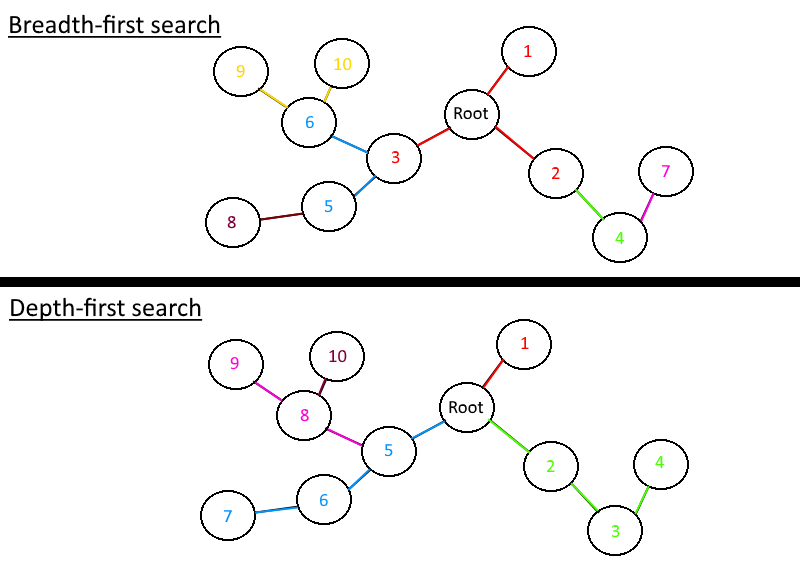
\includegraphics[width=\textwidth]{verschil-BFS-DFS.png}
  \caption{Schematische weergave van een willekeurige dataset.}
  \label{fig:verschil-BFS-DFS}
\end{figure}

In figuur \ref{fig:verschil-BFS-DFS} is de werking van BFS en DFS weergegeven. Het getal in elke node geeft aan als hoeveelste het bereikt wordt. 

Ook bij DFS hebben de nodes een state: bezocht of niet bezocht.
Ten eerste wordt de root gekozen en deze wordt als bezocht opgeslagen. Zoals te zien is wordt er vanaf de root \'e\'en (willekeurige) neighbour gekozen om te onderzoeken. Elke bezochte neighbour wordt als bezocht genoteerd. De root wordt in de stack geplaatst. Vanaf deze neighbour wordt weer een nieuwe aanliggende node gekozen, waarvan de state 'onbezocht' is. Ook nu wordt de bezochte node in de stack geplaatst. Dit proces herhaalt zich totdat er een node is zonder (onbezochte) neighbours. Op dat moment wordt de bovenste node uit de stack gehaald, dit heet backtracking, en herhaalt het proces zich. Dit blijft doorgaan totdat geen enkele node onbezochte neighbours over heeft of totdat het doel gevonden is.

Als vuistregel kan het volgende gehanteerd worden: depth-first search wordt gebruikt als je weet dat er maar \'e\'en uitkomst is, breadth-first search als je de makkelijkste of snelste uitkomst wil kiezen.

\subsection{Conclusie}
Twee voorbeelden van reguliere zoek algoritmes zijn "Breadth-first seach" en  "Depth-first search". Dit zijn twee algoritmes met vele toepassingen. Beide algoritmes zijn niet zelflerend omdat ze hun manier van zoeken niet zelf verbeteren.
\newpage

\textcolor{praktijk}{
\subsection{Praktijk: Voorbeelden algoritmes}
}
Algoritmes hebben meestal vele toepassingen. Hier zijn enkele voorbeelden van de eerder genoemde algoritmes.

\subsubsection{Breadth-first search}
\begin{figure}[h]
  \centering
    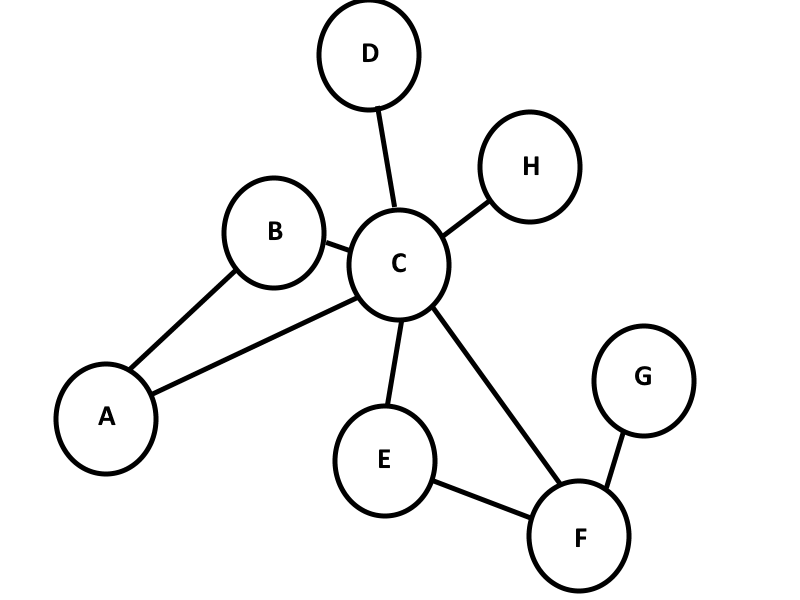
\includegraphics[width=0.8\textwidth]{datasetBFS2.png}
  \caption{Schematische weergave van een willekeurige dataset.}
  \label{fig:datasetBFS2}
\end{figure}

In figuur \ref{fig:datasetBFS2} is een dataset te zien, bijvoorbeeld een telefoonboom. Elke cirkel representeert \'e\'en persoon. Zo kan persoon A de personen B en C bellen, maar A bezit geen andere telefoonnummers. Toch zou hij een boodschap naar H kunnen sturen: via C. 
Stel, persoon A wil nu iets tegen F zeggen: in een kleine dataset als deze is het in \'e\'en oogopslag te zien dat de snelste manier hiervoor A – C – F is en dat A – B – C – E – F veel langer is. Bij grotere datasets is dit echter al snel moeilijk met zekerheid te zeggen. Hiervoor kan Breadth-first search ingezet worden.

\subsubsection{Depth-first search}

\begin{figure}[H]
  \centering
    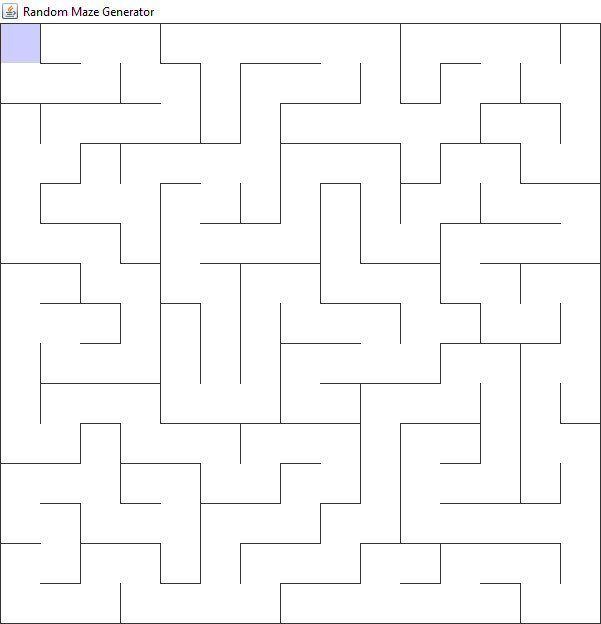
\includegraphics[width=0.8\textwidth]{maze.png}
  \caption{Een voorbeeld van een automatisch gegenereerd doolhof, gebruik makend van DFS.}
  \label{fig:maze}
\end{figure}

Depth-first search kan gebruikt worden voor zowel het maken als oplossen van doolhoven. In figuur \ref{fig:maze} is een doolhof te zien dat gemaakt is met behulp van DFS. Wij hebben in het kader van deze deelvraag een doolhof-generator gemaakt. Het algoritme in de vorm van een stappenplan is als volgt:

\begin{enumerate}
\item Kies een start cel en markeer deze als bezocht. Deze cel noemen we nu de \textit{current} cel.
\item Terwijl er nog niet bezochte cellen aanwezig zijn:
	\begin{enumerate}
	\item Als current neighbours heeft die nog niet bezocht zijn:
		\begin{enumerate}
		\item Kies willekeurig \'e\'en van de neighbours.
		\item Voeg current toe aan de stack.
		\item Verwijder de muur tussen de huidige cel en de gekozen cel.
		\item Benoem de gekozen cel als current en zet de state op bezocht.
		\item Kies willekeurig \'e\'en van de neighbours.
		\item Voeg current toe aan de stack.
		\item Verwijder de muur tussen de huidige cel en de gekozen cel.
		\item Benoem de gekozen cel als current en zet de state op bezocht.
		\end{enumerate}			
	
	\item Anders, als de stack niet leeg is:
		\begin{enumerate}
		\item Haal de laatst toegevoegde cel uit de stack en verwijder deze hieruit.
		\item Maak deze cel current.
		\item Haal de laatst toegevoegde cel uit de stack en verwijder deze hieruit.
		\item Maak deze cel current.
		\end{enumerate}	
	\end{enumerate}
\end{enumerate}


\newpage
\section{Wat zijn zelflerende algoritmes en waarin verschillen ze van reguliere algoritmes?}

\subsection{Machine learning}
Een zelflerend systeem is een algoritme gebaseerd op machine learning. Machine learning werd door Arthur Samuel, een pionier op dit gebied, gedefinieerd als: 
\textit{A field of study that gives computers the ability to learn without being explicitly programmed.} \cite{ArthurSamuel} 
In tegenstelling tot de eerder genoemde algoritmes is een zelflerend systeem in staat zichzelf te verbeteren. Hierdoor kan het taken uitvoeren waarbij reguliere algoritmes tekort schieten. Welke taken dit betreft, zullen we in de derde deelvraag behandelen. 

\begin{figure}[h]
  \centering
    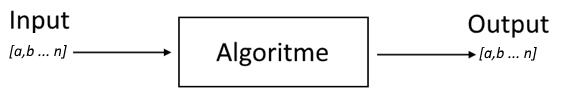
\includegraphics[width=\textwidth]{algorithm1.png}
  \caption{Schematische weergave van een zelflerend systeem}
  \label{fig:algorithm1}
\end{figure}

In figuur \ref{fig:algorithm1}  is een schematische weergave van een zelflerend systeem afgebeeld. Bepaalde input data gaat het systeem in en bepaalde output data komt het systeem uit. De input en output data bestaat uit \'e\'en of meerdere getallen. Als de input simpelweg een reeks getallen betreft, zal dit direct als input gebruikt kunnen worden. In het geval dat de input uit een ander datatype bestaat, zoals een plaatje, zal dit omgezet moeten worden in een reeks getallen voordat het in een zelflerend systeem gebruikt kan worden. Het algoritme zal deze getallen bewerken tot de gewenste output. Deze output wordt eveneens in getallen gegeven. Waar nodig zullen deze getallen dus weer moeten worden omgezet tot het gewenste datatype.

Er zijn veel verschillende algoritmes die gebruikt kunnen worden voor een zelflerend systeem. Elk algoritme heeft voor- en nadelen en is geschikt voor andere doeleinden. Een aantal van deze algoritmes zullen we in de tweede deelvraag behandelen. 

\subsection{Training}

Een zelflerend systeem begint in de meeste gevallen zonder enige kennis van de data. Om de gewenste output te kunnen produceren is het dus nodig om het systeem eerst input data te geven zodat het kan leren. Dit proces wordt het \textbf{trainen} genoemd. Voor het trainen van een zelflerend systeem is training data nodig. Deze data moet gelijk of gelijkwaardig zijn aan de \textit{echte} data. De training data kan in veel verschillende vormen voorkomen en de manier van trainen is afhankelijk van de vorm van de (training) data. In figuur \ref{fig:algorithm2}  is te zien dat het trainen los staat van het algoritme. Dit verschil zullen we in de volgende deelvraag wat duidelijker maken. 
Er zijn drie prominente manieren waarop een zelflerend systeem getraind kan worden: \textbf{supervised}, \textbf{unsupervised} en \textbf{reinforcement learning}.

\begin{figure}[H]
  \centering
    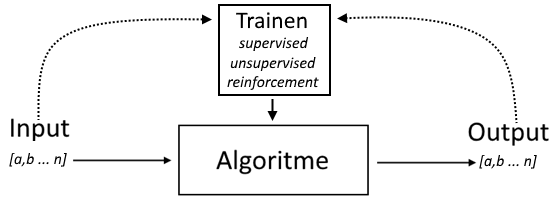
\includegraphics[width=\textwidth]{algorithm2.png}
  \caption{Schematische weergave van een zelflerend systeem}
  \label{fig:algorithm2}
\end{figure}

\subsubsection{Supervised Learning}
In het geval van supervised learning heb je te maken met \textbf{labeled} training data. Anders gezegd: van een bepaalde input is de gewenste output al bekend. Een klassiek voorbeeld van een labeled dataset is een dataset van huisprijzen en huiseigenschappen (zie figuur \ref{fig:LabeledDataset})

\begin{table}[h]
\centering
\begin{tabular}{llll}
\hline
\multicolumn{1}{c}{\multirow{2}{*}{Huisprijs (output)}} & \multicolumn{3}{c}{Huiseigenschappen (input)} \\
\multicolumn{1}{c}{} & \multicolumn{1}{c}{Woonoppervlakte} & \multicolumn{1}{c}{Perceeloppervlakte} & \multicolumn{1}{c}{Aantal Kamers} \\ \hline
€ 519.000 & 124 m² & 311 m² & 4 \\
€ 569.000 & 133 m² & 309 m² & 5 \\
€ 569.500 & 170 m² & 310 m² & 6 \\ \hline
\end{tabular}
\caption{Labeled dataset Bron: http://www.funda.nl/koop/huizen/ }
\label{fig:LabeledDataset}
\end{table}
Bij de training dataset van tabel \ref{fig:LabeledDataset} is de gegeven input de huiseigenschappen en de gewenste output de huisprijs. Het systeem wordt met deze dataset getraind. Hierdoor leert het een output te produceren die steeds dichter bij de gewenste output ligt. Als er een verband bestaat tussen de huiseigenschappen en de huisprijs, wat waarschijnlijk het geval is, zal het zelflerende systeem na genoeg trainen in staat zijn zelf bij nieuwe huiseigenschappen een huisprijs te voorspellen. \cite{MLCourse1}

\subsubsection{Unsupervised Learning}
Unsupervised learning kan gebruikt worden bij een \textbf{unlabeled} dataset ofwel, een dataset waarbij de data niet geclassificeerd is en er geen gewenste output bekend is. Als je een dataset hebt van heel veel niet-geordende foto's is het niet mogelijk om dit te classificeren. Als een deel van de dataset gelabeld wordt, zal met behulp van supervised learning de rest van de dataset geclassificeerd kunnen worden. Dit is echter in veel gevallen niet mogelijk, bijvoorbeeld doordat de dataset enorm groot is of er zodanig veel verschillende groepen bestaan dat het menselijk niet mogelijk is ook maar een deel te labelen. Ook kan het zo zijn dat men niet weet of er een verband aanwezig is. 
Kortom: unsupervised learning wordt gebruikt voor het classificeren van data, zonder dat er groepen vooraf gedefinieerd zijn. Met behulp van deze vorm van training zullen in een grote dataset verbanden kunnen worden ontdekt, die men misschien niet zonder hulp had kunnen achterhalen.\cite{MLCourse2}

\subsubsection{Reinforcement Learning}
Reinforcement learning is een zeer specifieke soort van leren. Er is bij deze vorm van learning geen dataset met input data, maar is er een bepaalde \textbf{context}. In deze context bevindt zich een \textbf{agent}. Een agent is een object dat bepaalde opdrachten kan uitvoeren. De context is een wereld waarin deze agent zich bevindt. Door de agent bij bepaalde acties pluspunten of minpunten te geven kun je bepaald gedrag bevorderen.  

\begin{figure}[h]
  \centering
    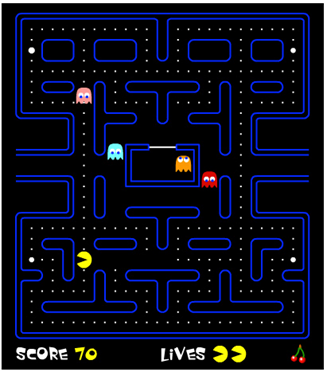
\includegraphics[width=0.5\textwidth]{pacman.png}
  \caption{Pacman}
  \label{fig:Pacman}
\end{figure}

In figuur \ref{fig:Pacman} is het spel Pac-Man te zien. Op dit spel zou reinforcement learning toegepast kunnen worden. De agent is hierbij pacman, dit is namelijk een object dat bepaalde opdrachten kan uitvoeren, zoals: beweeg naar links. De context is hierbij het level, ofwel: de positie van de muren (de blauwe obstakels), de posities van de ghosts (de gekleurde vijanden), de posities van de pac-dots (de kleine stipjes) en de posities van de power-pellets (de grotere stipjes). [4] Het eten van de pac-dots is positief, het geraakt worden door de ghosts is negatief. Door reinforcement learing toe te passen op het spel zal de agent steeds beter worden in het spelen van het spel. 

\subsection{Normaliseren van data}
Zoals ook in tabel \ref{fig:LabeledDataset} te zien is, kunnen verschillende inputs erg van elkaar verschillen qua grootte. Zo zal het aantal kamers nooit in de buurt komen van het oppervlak. Uiteindelijk zou dit een probleem kunnen veroorzaken bij de berekeningen van het systeem. Een groot getal zou namelijk een veel groter aandeel kunnen hebben alleen omdat het getal zoveel groter is. Het is daarom gebruikelijk de inputs te normaliseren. Dit houdt in dat de inputs zullen veranderen in een getal met een waarde binnen een bepaald gebied zodat alle verschillende inputs eerlijk met elkaar vergeleken kunnen worden. Je zou bijvoorbeeld voor de oppervlaktes kunnen stellen dat alle waardes tussen 100 m² en 1000 m² zullen liggen. Aan een input van 500 m² zou je dan een waarde van 5 kunnen geven.

\subsection{Conclusie}
Zelflerende computersystemen zijn algoritmes gebaseerd op machine learning. Een zelflerend systeem verschilt van reguliere algoritmes zoals breadth-first search en depth-first search doordat ze in staat zijn zichzelf te verbeteren.


\newpage
\section{Machine learning algoritmes}
\label{chapter:MLA}

\subsection{Inleiding}
In het vorige hoofdstuk hebben we behandeld wat een zelflerend systeem is. In dit hoofdstuk gaan wij dieper in op de verschillende soorten zelflerende algoritmes en beantwoorden we de vraag: \textit{Wat zijn voorbeelden van zelflerende algoritmes en hoe werken ze?} We zullen in deze deelvraag naar drie verschillende algoritmes kijken: \textit{Linear Regression, Support vector machines en Artificial Neural Networks.} \cite{SunilRay} 

\subsection{Linear Regression}
Het eerste machine learning algoritme dat we gaan behandelen is \textbf{linear regression}. Dit algoritme wordt gebruikt voor het voorspellen van een y-waarde bij gegeven x-waarde(n). Om linear regression te kunnen gebruiken is het belangrijk dat er wel een lineair verband bestaat tussen de x-waarde(n) en de y-waarde. In figuur \ref{fig:LinearRegression1} is een dergelijk linear verband te zien. 
Dit lineaire verband is te beschrijven met de formule:
\textit{y = ax + b}

\begin{figure}[h]
  \centering
    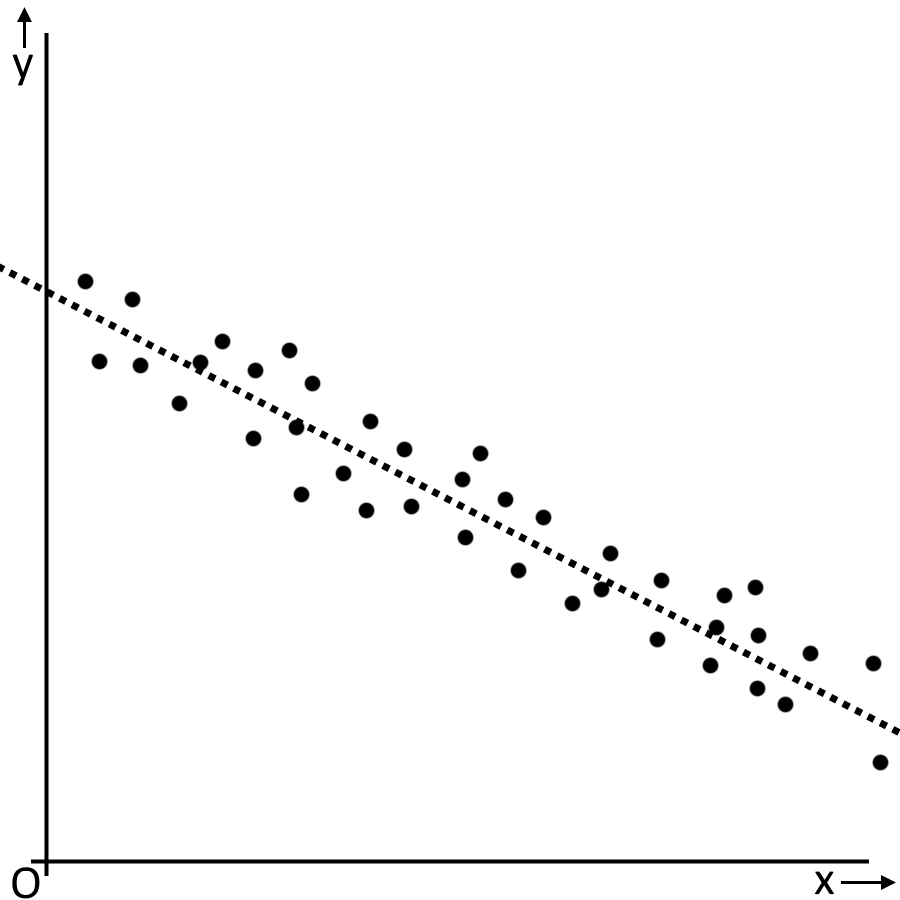
\includegraphics[width=0.5\textwidth]{linearRegression.png}
  \caption{Linear regression}
  \label{fig:LinearRegression1}
\end{figure}

Het doel bij linear regression is het bepalen van de waarde voor a en b. Dit is op verschillende manieren mogelijk. Een statistische manier hiervoor is door gebruik te maken van het \textbf{ordinary least squares} algoritme. Dit algoritme bepaalt de best passende lijn door de punten, ook wel bekend als de trendlijn. De waarden voor a en b worden hierbij als volgt bepaald:

\begin{align*}
	a&=\frac{\sum_{i=0}^{n}(x_{i}-\bar{x})(y_{i}-\bar{y})}{\sum_{i=0}^{n}{(x_{i}-\bar{x}})^{2}}\\
	b&=\bar{y}-(a * \bar{x})
\end{align*}

In deze formules is $\bar{x}$ het gemiddelde van alle x-waarden en de $\bar{y}$ het gemiddelde van alle y-waarden. 
Dit algoritme is echter alleen toepasbaar als er sprake is van \'{e}\'{e}n x-waarde als invoer, dus geen multidimensionale invoer waarden zoals $(3,3)$. Bij meerdere x-waarden is dit algoritme dus niet te gebruiken. Een andere manier om de a en b waarde te vinden is door gebruik te maken van een leerstrategie. In deelvraag 4 bespreken we drie verschillende leer strategieën.

\subsection{Support vector machine}
Een support vector machine (SVM) is een machine learning algoritme ontwikkeld door Vladimir Vapnik. Het algoritme kan gebruikt worden voor het classificeren van data. Het algoritme is een vorm van supervised learning. \cite{SVM}

\begin{figure}[h]
  \centering
    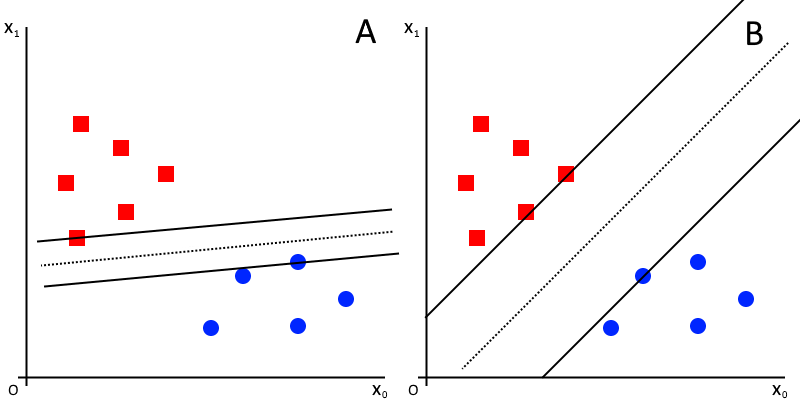
\includegraphics[width=0.5\textwidth]{SVM.png}
  \caption{Support vector machines}
  \label{fig:SupVectorMachine1}
\end{figure}

Een support vector machine werkt als volgt: Het trekt een lijn, een \textbf{vector}, tussen de twee groepen. Deze vector is z\'o dat \textit{de afstand tussen de vector en het dichtstbijzijnde datapunten zo groot mogelijk is.} \cite{SVM2} Deze dichtstbijzijnde datapunten worden de \textbf{support vectoren} genoemd In figuur \ref{fig:SupVectorMachine1} is twee keer dezelfde dataset weergegeven. In de linker afbeelding is te zien dat de vector de twee groepen scheidt maar de afstand tussen het dichtstbijzijnde datapunt kleiner is dan bij de rechter afbeelding, deze afstand wordt de marge genoemd. De in de rechter afbeelding is de marge het grootst, dus dit is de betere vector. Het gebied tussen de twee support vectoren wordt het \textbf{hyperplane} genoemd.

\subsubsection{Het agoritme}
Het doel van het algoritme is van een nieuw datapunt bepalen of het tot groep A (de rode vierkantjes) of groep B (de blauwe cirkels) behoort. Als een nieuw datapunt behoort tot groep A dan willen we dat de output van het algoritme negatief is en als het nieuwe datapunt behoort tot groep B willen we dat de output positief is. Hoe positiever of negatiever de output is hoe zekerder het is dat dit punt daadwerkelijk tot die groep behoort. Als de output 0 is, dan bevindt het punt zich precies tussen de twee groepen, het ligt dan op de stippellijn van figuur \ref{fig:SupVectorMachine1}. Verder is het zo dat de output tussen -1 en 1 ligt als het binnen de twee support vectoren ligt. In dit gebied is het niet helemaal zeker tot welke groep het punt behoort. 
We kunnen de drie vectoren als volgt definiëren: 

\begin{center}
De linker support vector	\textit{w * x - b = -1}
\\De middelste vector			\textit{w * x - b = 0}
\\De rechter support vector 	\textit{w * x - b = 1}
\end{center}

Een support vector machine probeert het volgende:

\begin{itemize}
\item Alle datapunten moeten buiten de twee support vectoren liggen
\item De afstand tussen de support vectoren moet zo groot mogelijk zijn
\end{itemize}

Vanuit de vectoren zijn de volgende twee formules af te leiden:
\begin{itemize}
\item De formule voor of een datapunt buiten de twee support vectoren ligt: $y_{i}(w^{T}x_{i} - b) \geq 0 $
\item De formule voor de afstand tussen de twee support vectoren: $\frac{2}{||w||}$
\end{itemize} 

Een vector die voldoet aan de volgende eisen wordt gekozen:
\begin{itemize}
\item Voor alle datapunten moet gelden: $y_{i}(w^{T}x_{i} - b) \geq 0 $
\item $\frac{2}{||w||}$ moet zo klein mogelijk zijn, ofwel $||w||$ zo groot mogelijk
\end{itemize}



\subsubsection{Kernel Methods}
In veel gevallen zal de dataset niet zo mooi geordend zijn als in figuur \ref{fig:SupVectorMachine1}. Het is dan niet mogelijk om een rechte lijn te trekken die de twee groepen scheidt. Een support vector machine zou in dit geval dus niet werken. Om toch een support vector machine te kunnen gebruiken is er iets genaamd de \textbf{kernel krick}.

\begin{figure}[h]
  \centering
    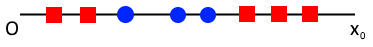
\includegraphics[width=0.5\textwidth]{dataset1d.png}
  \caption{Een één dimensionale dataset}
  \label{fig:SupVectorMachine2}
\end{figure}

In figuur \ref{fig:SupVectorMachine2} is een \'{e}\'{e}n dimensionale dataset te zien, dit wil zeggen, er is maar \'{e}\'{e}n variabele. Met een support vector machine is het nu niet mogelijk om een lijn te trekken die de twee groepen scheidt. Daarom wordt er een extra variabele bij gemaakt, bijvoorbeeld $X_{1} = (X_{0})^{2}$. Nu is het wel mogelijk een lijn te trekken door de dataset die de twee groepen opdeelt:

\begin{figure}[h]
  \centering
    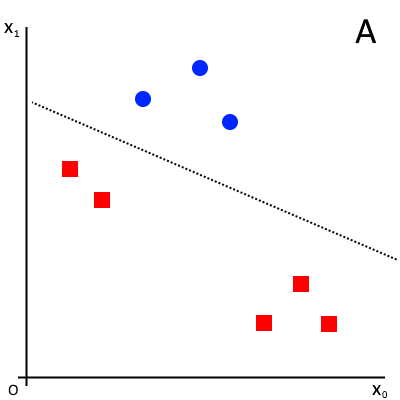
\includegraphics[width=0.5\textwidth]{KernelMethod.png}
  \caption{Een dataset, met een fictief uitgevoerde kernal trick, gescheiden door een lijn}
  \label{fig:SupVectorMachine2}
\end{figure}

\subsection{Artificial Neural Networks}
\subsubsection{Biologisch en kunstmatig netwerk}
Binnen mensen wordt informatie overgebracht door middel van het zenuwstelsel. Dit zenuwstelsel is opgebouwd uit miljarden zenuwcellen. Een zenuwcel, ook wel een neuron genoemd, is opgebouwd uit drie delen: een cel lichaampje, een aantal dendrieten en \'{e}\'{e}n axon. In firguur \ref{fig:BiologischNeuron} is een weergave van een biologische neuron te zien.

\begin{figure}[h]
  \centering
    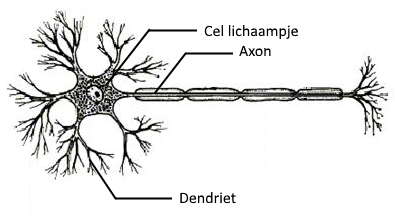
\includegraphics[width=0.5\textwidth]{BiologischNeuron.png}
  \caption{Een tekening van een biologisch neuron}
  \label{fig:BiologischNeuron}
\end{figure}

In de biologie zijn dendrieten verantwoordelijk voor de instroom van informatie, zij brengen informatie (impulsen) naar het cel lichaampje toe. De zenuwcel kan deze informatie vervolgens via een enkele axonen doorgeven aan een dendriet van een andere zenuwcel of aan een spier. Het doorgeven van informatie gebeurt in het uiteinde van de axon en dendrieten, in zogeheten synapsen.

Het principe van een neuron kan ook door een computer uitgevoerd worden. Dit is het idee voor een Artificial Neural Network (ANN). Een dergelijk netwerk bestaat uit een verschillend aantal ‘computerneuronen’. Elk van deze neuronen krijgt, net zoals een biologische neuron, informatie binnen. Binnen de neuron vindt een berekening plaats. Vervolgens wordt deze waarde doorgegeven aan de volgende neuron of gegeven als output.

\subsubsection{De perceptron}
De simpelste vorm van een neural network is een netwerk met slechts \'{e}\'{e}n neuron. Zo'n ANN, voor het eerst gemaakt door  F. Rosenblatt in 1958 \cite{ANN1}, wordt een \textbf{perceptron} genoemd.

\begin{figure}[h]
  \centering
    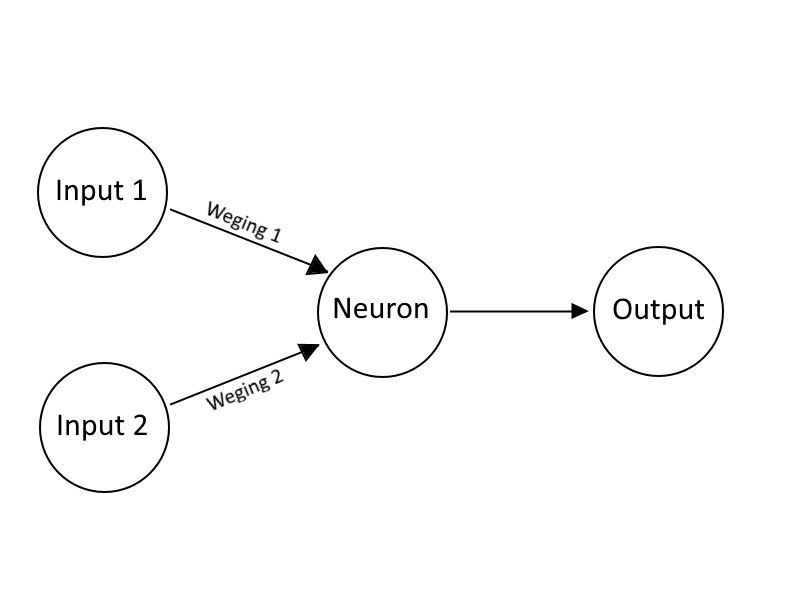
\includegraphics[width=0.5\textwidth]{Perceptron.png}
  \caption{een schematische weergave van en perceptron}
  \label{fig:perceptron}
\end{figure}

In figuur \ref{fig:perceptron} is te zien dat een neuron twee inputs binnen krijgt en daarna een output geeft. De pijlen naar de neuron toe en er vanaf stellen de synapsen voor. Elke synaps heeft een bepaalde weging. De weging van een synaps bepaald hoeveel invloed die ene input heeft op het netwerk. Het uiteindelijke doel van een neural network is \textit{het zoeken naar de optimale weging voor alle synapsen binnen het netwerk.} 
Om tot een output te kunnen komen moet de neuron een berekening uitvoeren. In deze situatie is de berekening nog vrij eenvoudig:

\begin{center}
$ Som van inputs = X_{1} * W_{1} + X_{2} * W_{2}$
\end{center}

\subsubsection{Activation functions}
De waarde die uit deze berekening volgt, wordt door een \textbf{activation function} gehaald. Een activation function zorgt ervoor dat aan deze som een waarde kan worden gehangen, bijvoorbeeld 1 of -1, zonder dat de som absoluut deze waarde heeft. Dit wordt gedaan door te kijken waar het punt op de grafiek van deze functie zich bevind.

\begin{figure}[h]
  \centering
    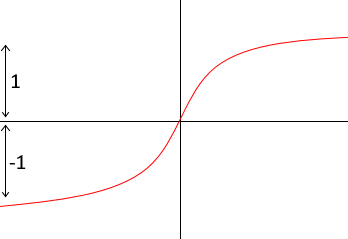
\includegraphics[width=0.5\textwidth]{GenericActivationFunction.png}
  \caption{Een voorbeeld van een algemene activation function en welke waardes hieraan worden gekoppeld.}
  \label{fig:actFunction}
\end{figure}

In figuur \ref{fig:actFunction} is een grafiek van een activation function gegeven. In dit voorbeeld worden aan alle positieve y waardes een 1 verbonden en aan alle negatieve een -1.

Een ANN is een vorm van supervised learning. Het programma weet dus wat het antwoord zou moeten worden. Als de output correct is zal er weinig gebeuren, maar als de output incorrect is zal het programma zichzelf moeten aanpassen om wel de goede uitkomst te krijgen. Dit gebeurt met behulp van de wegingen van elke synaps. Deze wegingen kunnen namelijk worden aangepast. De invloed van elke input kan ofwel vergroot ofwel verkleint worden. Op deze manier zal uit de berekening in de neuron de volgende keer misschien een andere, betere uitkomst komen. De nieuwe weging van een synaps wordt nu:$ w_{0} = w_{1} + ∆w $.
Hoe ∆w berekend wordt, wordt bepaald door de leerstrategie van het systeem. Hier wordt in de volgende deelvraag verder op in gegaan.

\subsubsection{Bias}
Met de besproken perceptron is echter een probleem. Wanneer beide inputs gelijk zijn aan nul heeft het aanpassen van wegingen geen effect. Een weging maal nul zal immers altijd in nul resulteren. Om dit probleem tegen te gaan, wordt er een \textbf{bias} toegevoegd. Dit is een extra input die standaard gelijk is aan \'{e}\'{e}n. De weging van de synaps van de bias wordt niet veranderd. Omdat de neuron nu ook bij inputs van nul een andere uitkomst uit de berekening zal geven, zal er nu toch een getal door de activation function gaan en zullen de wegingen toch worden aangepast. 

\subsubsection{Een netwerk van perceptrons}
Natuurlijk is het ook mogelijk van niet \'{e}\'{e}n, maar meerdere perceptrons te hebben. Zo wordt het een echt netwerk van synapsen en neuronen.

\begin{figure}[h]
  \centering
    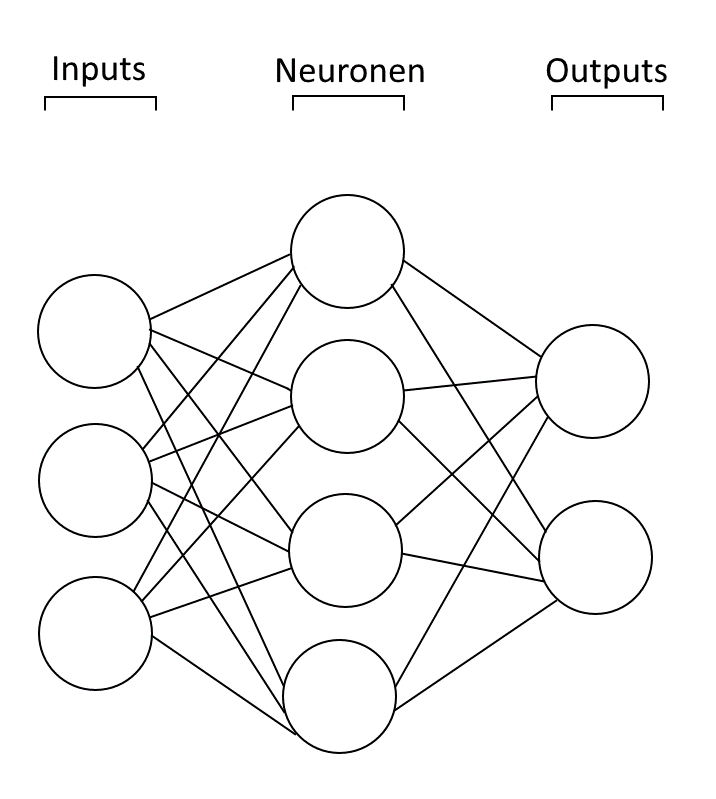
\includegraphics[width=0.5\textwidth]{GenericNeuralNetwork.png}
  \caption{Een schematische weergave van een willekeurig ANN.}
  \label{fig:ANN}
\end{figure}

Ook is het mogelijk meerdere lagen neuronen te hebben. Dit wordt een \textbf{deep neural network} genoemd, of simpelweg \textbf{deep learning}.
De tot nu toe besproken ANN’s hebben hun informatie allemaal in \'{e}\'{e}n richting bewogen: van alle inputs, naar alle neuronen, naar alle outputs. Dit wordt \textbf{feedforward} genoemd. Ook zou je een neural network kunnen hebben waarin de informatie ook nog tussen de neuronen in dezelfde laag beweegt: een \textbf{recurrent neural network}.

\subsection{Conclusie}
Voorbeelden van zelflerende algoritmes zijn: \textit{Linear regression}, \textit{Support vector machines} en \textit{Arteficial Neural Networks}. Alle drie de algoritmes werken verschillend en zijn goed voor verschillende scenario's. Linear regression werkt door het opstellen van een lineare formule door waarden met een linear verband. Support vector machines werken door een vector te maken die twee groepen zo goed mogelijk scheidt. En Arteficial neural networks werken door een netwerk van neuronen te simuleren.


\newpage
\section{Op wat voor manieren kunnen zelflerende algoritmes zichzelf verbeteren?}

\subsection{Inleiding}
In de vorige deelvraag hebben we verschillende Machine Learning algoritmes behandeld. Hierbij hebben we nog niet besproken hoe een algoritme zichzelf kan verbeteren: Hoe bepalen we bij Linear Regression de waarden voor a en b in de formule $ y = ax + b $? Hoe bepalen we de waarden voor  x en b in de vector $ w ∙ x - b = 0 $ bij een Support Vector Machine? Hoe bepalen we de wegingen van de synapsen in een Artificial Neural Network? Er zijn verschillende manieren waarop al deze waarden bepaald kunnen worden: Gradient Descent, Newton's method en evolutionary improvement. Deze drie leerstrategieën zullen we in deze deelvraag behandelen.

\subsection{Gradient descent}
De eerste leerstrategie die we behandelen is gradient descent. Gradient descent is een algoritme dat functies minimaliseert. Door het aanpassen van bepaalde parameters wordt geprobeerd de waarde van een bepaalde functie zo laag mogelijk te maken. De functie die we bij een zelflerend systeem proberen te minimaliseren is de cost function, ook wel loss function genoemd. Dit is een functie die bepaalt hoe goed het systeem op dat moment werkt. Er wordt bepaald hoeveel de huidige outputs afwijken van de gewenste outputs. Het is hierbij dus nodig dat je de gewenste outputs weet bij gegeven inputs. Er is dus bij gradient descent altijd sprake van supervised learning. 

\subsubsection{Het algoritme} 
\begin{figure}[h]
  \centering
    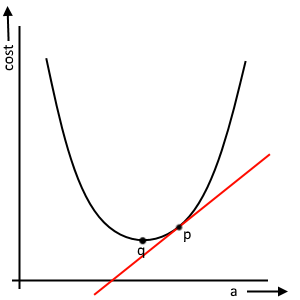
\includegraphics[width=0.5\textwidth]{GenericCostFunction.png}
  \caption{De cost function}
  \label{fig:GenericCostFunction}
\end{figure}

In figuur \ref{fig:GenericCostFunction} is de cost van een bepaalde situatie uitgezet tegen een variabele a. Dit kan bijvoorbeeld de a uit de formule $ y = ax + b $ bij Linear Regression zijn.  Het is dus te zien dat de cost minimaal is in punt q. We willen dus dat a gelijk wordt aan de waarde van a in punt q. Nu is dit punt in deze grafiek erg makkelijk te vinden, maar zodra er gebruik wordt gemaakt van ingewikkeldere algoritmen, zoals een ANN, wordt dit punt moeilijker te bepalen.

Op een gegeven moment in het trainingsproces is de a gelijk aan het punt p. Het Gradient Descent algoritme doet dan het volgende:
\begin{itemize}
\item De afgeleide op het huidige punt wordt bepaald (de rode lijn in figuur \ref{fig:GenericCostFunction}).
\item De a wordt zodanig aangepast dat het meer in de richting komt van de q. (Dit wordt gedaan door de afgeleide bij de variabele op te tellen)
\end{itemize}

Wanneer Gradient Descent wordt toegepast zal een bepaalde variabele in een zelflerend systeem zo aangepast worden dat de cost als gevolg van die variabele het laagst wordt. 

\subsubsection{De wiskunde achter gradient descent}
Het Machine Learning algoritme produceert met een bepaalde input een bepaalde output, dit noemen we de \textbf{guess}. Omdat we weten wat de goede ouput is kunnen we de \textbf{error} bepalen voor die input. De goede output in de volgende formule is y.

\begin{center}
$ error_{i} = y_{i} - guess_{i}$
\end{center} 

De vorige formule geldt dus voor de individuele datapunten. De totale error, de som van alle individuele error waarden, ook wel cost of loss genoemd kan als volgt beschreven worden:

\begin{center}
$ cost = \sum_{i=0}^n(error_i)^2$
\end{center}

Zoals bekend uit de wiskunde is het mogelijk om hiervan de laagste waarde te bepalen door de afgeleide op nul te herleiden. Voor elk individueel datapunt is de afgeleide van de error:

\begin{center}
$ cost' = 2(error_i) * error'_i$
\end{center}

Bij het differentiëren wordt gebruik gemaakt van de kettingregel.

\subsubsection{Linear regression met gradient descent}
Om het principe van Gradient Descent beter te begrijpen gaan we nu doormiddel van Gradient Descent Linear Regression uitvoeren.

De guess is hier dus de huidige uitkomst van $ y = ax + b $.

\begin{center}
$ error_{i} = y_{i} - (xa + b)_{i}$
\end{center}

De waarde van $ b_{i} $, $ x_{i} $ en $ y_{i} $ zijn hier constant. De $ x_{i} $ en $ y_{i} $ zijn namelijk bekend uit de training data en $ b_{i} $ veranderd wel, maar niet hierbij. De afgeleide van de error functie is dan:

\begin{center}
$ error'_{i} = x$
\end{center}

De afgeleide van de cost function is dan:
\begin{align}
cost' &= 2(error) * x \\
cost' &= 2(y_{i} - (xa + b)_{i}) * x
\end{align}

Met de deze afgeleide is de helling van de cost function te bepalen. Hiermee dus te bepalen welke richting we de variabele a in moeten veranderen. Het aanpassen van de a bij Linear Regression gebeurd dus als volgt:

\begin{center}
$ a = a + (2 * error * x)$
\end{center}

\subsubsection{Learning rate}
Een zelflerend systeem bereikt niet in een keer de gewenste output. Er wordt langzaam in de richting van de goede output gewerkt. De formule voor het aanpassen van de a waarde uit het vorige kopje is daarom iets anders. Er wordt een \textbf{learning rate} geïntroduceerd:

\begin{center}
$ a = a + (error * x * learning rate)$
\end{center}

Het kiezen van een goede learning rate is heel belangrijk. Een te lage learning rate zorgt ervoor dat het heel lang duurt voordat de goede output bereikt wordt. Een te hoge learning rate zorgt ervoor dat de gewenste output voorbij wordt geschoten. De gewenste output wordt dan nooit bereikt omdat de variabele net te groot of te klein wordt gemaakt. \cite{GradientDescent1}\cite{GradientDescent2}

\subsection{Newton's method}
Net zoals gradient decent is Newton’s method, vernoemd naar Isaac Newton, een manier om de laagste waarde van een bepaalde functie te bepalen. Hiervoor maakt gradient descent gebruik van het gegeven dat een extreme waarde van een grafiek een richtingsco\"effici\"ent van 0 heeft en de afgeleide op dat punt dus gelijk is aan 0. Newton’s method gebruik voor het bepalen van de laagste waarde de tweede afgeleide. Er wordt dan gekeken op welke punten deze lijn de x-as snijdt, dit zijn namelijk de toppen van de grafiek van de eerste afgeleide. Door gebruik te maken van Newton’s method, zal je een schatting krijgen van het snijpunt met de x-as, maar waarschijnlijk zal je dit punt niet exact kunnen vinden. De nauwkeurigheid van de schatting hangt af van de hoeveelheid waarmee je de stappen herhaalt.

\subsubsection{Het proces}
In figuur \ref{fig:NM1} is een willekeurige grafiek getekend.

\begin{figure}[H]
  \centering
    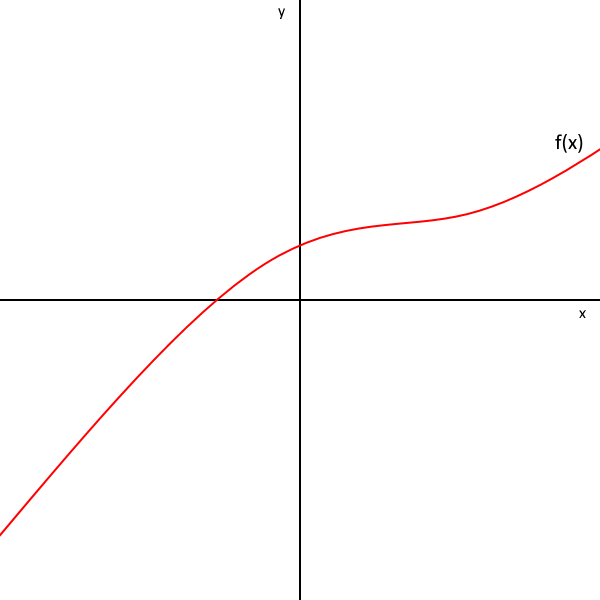
\includegraphics[width=0.5\textwidth]{NewtonsMethod1.png}
  \caption{De grafiek van een willekeurige functie $ f(x) $}
  \label{fig:NM1}
\end{figure}

Bij het gebruik van Newton’s method, waarbij we dus zoeken naar een snijpunt met de x-as, wordt eerst een gok gedaan. Deze gok, op punt a, correspondeert met een waarde op de grafiek van $ f(x) $. Aan dit punt wordt een raaklijn getekend.

\begin{figure}[h]
  \centering
    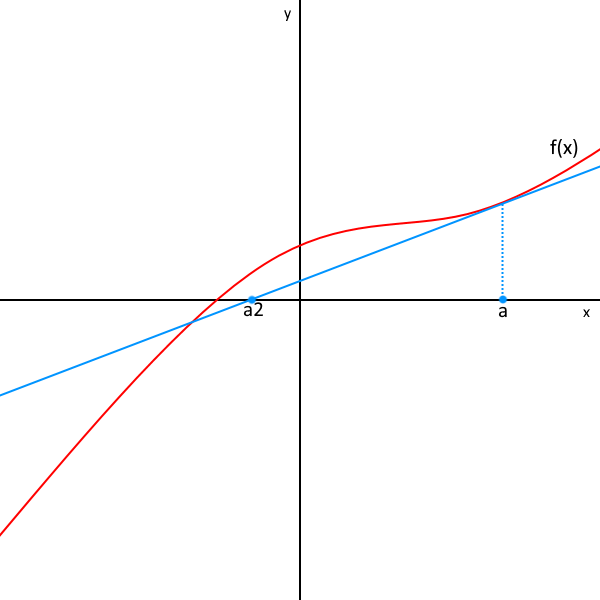
\includegraphics[width=0.5\textwidth]{NewtonsMethod2.png}
  \caption{Een raaklijn aan $ f(x) $ op punt $ x = a $}
  \label{fig:NM2}
\end{figure}

De raaklijn van $ f(x) $ op $ f(a) $ snijdt de x-as op een bepaald punt $ a_2 $. Te zien is dat dit punt al aanzienlijk dichten bij het doel ligt dan de originele schatting. Ook $ a_2 $ correspondeert met een waarde van $ f(x) $ en ook op dit punt kan weer een raaklijn getekend worden.

\begin{figure}[h]
  \centering
    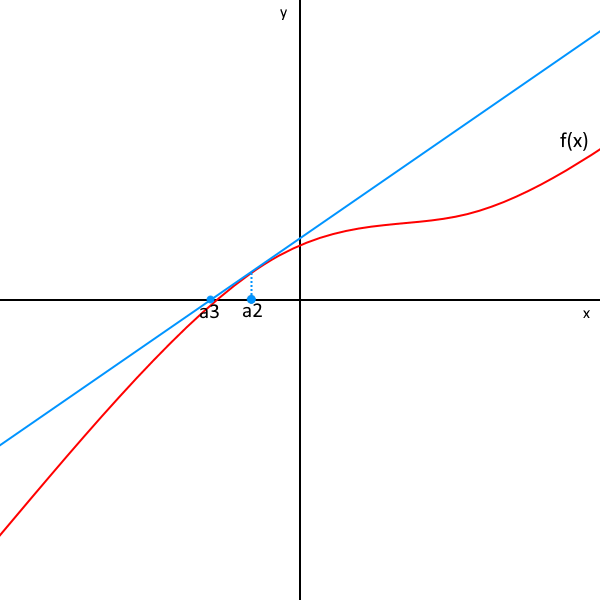
\includegraphics[width=0.5\textwidth]{NewtonsMethod3.png}
  \caption{Een raaklijn aan $ f(x) $ op punt $ x = a_2 $}
  \label{fig:NM3}
\end{figure}

Na slechts twee raaklijnen getekend te hebben, ligt het punt $ a_3 $ al erg dicht bij het doel. Om een nauwkeurigere benadering van dit doel te bereiken kan je vaker een raaklijn tekenen en het nieuwe snijpunt bepalen. Hoe nauwkeurig je een benadering wil hebben verschilt per situatie.

\subsubsection{De wiskunde}
Uiteraard zijn de waardes van de punten $ a_2 $, $ a_3 $ … $ a_n $ te berekenen, we willen immers de waarde van het nulpunt bepalen. Dit gebeurt als volgt:

We weten dat de afgeleide de helling van de grafiek aangeeft: $ \frac{\Delta y}{\Delta x} $. Het idee is dat je de helling berekent tussen twee punten die oneindig dicht bij elkaar liggen, hier aangegeven met d: $ \frac{dy}{dx} $. Voor het gemak noemen we deze punten x en c. Dit geeft voor de afgeleide:

\begin{center}
$ f'(c) = \frac{f(x) - f(c)}{x - c}$
\end{center}

Dit kan omgeschreven worden tot de formule voor een raaklijn:

\begin{align}
	   f'(c)(x - c) &= f(x) - f(c) \\
f'(c)(x - c) + f(c) &= f(x)
\end{align}

Om het nulpunt te berekenen moet gelden f(x)=0. Omdat c slechts een andere waarde voor x aanduidde, kunnen we deze vervangen door het volgende:$ c = x_n $ en $ x = x_{n+1} $

\begin{align}
			 f'(x_n)(x_{n+1} - x_n) + f(x_n) &= 0 \\
	f'(x_n)* x_{n+1} - f'(x_n) * x_n + f(x_n)&= 0 \\
							f'(x_n)* x_{n+1} &= f'(x_n) * x_n - f(x_n) \\
		   \frac{f'(x_n) * x_{n+1}}{f'(x_n)} &= \frac{f'(x_n) * x _n - f(x_n)}{f'(x_n)} \\
									  x_{n+1}&= x_n - \frac{f(x_n)}{f'(x_n)}
\end{align}




Met deze formule kan de volgende waarde voor x berekend worden.

\subsubsection{Het gebruik}
Er zijn vele situaties te bedenken waarin je de nulpunten van een functie zou willen weten. In het gebied van machine learning wordt het gebruikt om te berekenen waar de cost functie minimaal is. Onder het kopje gradient descent staat al beschreven hoe we aan de cost functie komen en wat de afgeleide hier van is. De grafiek die afgebeeld staat zou de afgeleide van deze cost functie zijn. Dit betekent namelijk dat de tweede afgeleide van de cost functie wordt genomen wanneer je een raaklijn aan de grafiek berekent.

Gradient descent kan goed worden gebruikt bij grafiek met slechts \'e\'en minimum. Zodra dit niet het geval is, kan het makkelijk in een dal vast blijven hangen, denkend dat het de minimale waarde gevonden heeft, terwijl er misschien nog een lager punt te vinden is. Bij zulke gevallen kan Newton’s method ingezet worden, want al deze punten zullen wel op de x-as liggen en dus zullen ze allemaal te vinden zijn met Newton’s method.

\subsection{Evolutionary improvement}
Het leerproces van een systeem zou de evolutie van het systeem genoemd kunnen worden, het leert zichzelf beter te functioneren in een omgeving. Net zoals evolutie in de biologie, gaat evolutionary improvement in generaties van systemen. Deze manier van leren maakt gebruik van het doorgeven van informatie tussen deze generaties om het algemene niveau van presteren te verhogen.

\subsubsection{DNA}
Wanneer evolutionary improvement wordt toegepast, is er altijd sprake van een bepaald DNA. In dit DNA staan een aantal waardes. Deze waardes kunnen worden doorgegeven aan de volgende generatie.

\subsubsection{Een populatie}
Wanneer de informatie van een enkel individu telkens wordt doorgegeven aan een volgende generatie die ook bestaat uit slecht één individu, zal de verbetering van een systeem niet zo groot of zelfs afwezig zijn. Het systeem weet niet of het DNA dat doorgegeven wordt goed of slecht presteert, want er is maar één individu per generatie. Om deze reden bestaat een generatie meestal uit meerdere individuen. Ze zullen niet allemaal even goed presteren en dus zal er onderscheid gemaakt kunnen worden tussen goed en slecht.

Hoe de overgave van DNA wordt geregeld kan op veel verschillende manieren en is afhankelijk van het soort programma en de voorkeur van de programmeur. Je zou bijvoorbeeld de individuen uit een populatie kunnen rangschikken op volgorde van prestatie (hoe prestatie wordt gemeten is natuurlijk ook geheel afhankelijk van het soort programma) en een bepaald percentage van het slechtst presterende deel laten afvallen \cite{carrykh}. Vervolgens vul je dit deel weer op met individuen met een willekeurig DNA, de rest van de populatie blijft gelijk. Het idee is dat je door telkens het slechte DNA weg te filteren, uiteindelijk een populatie krijgt die gemiddeld steeds beter presteert.

Een andere manier voor evolutie is stellen dat na een bepaalde tijd elk individu een ‘kind’ krijgt. Dit zou goed kunnen werken in een simulatie waarin individuen een rivaliserend verband met elkaar hebben, bijvoorbeeld doordat ze dezelfde voeding nodig hebben. De individuen die langer overleven zullen meer kinderen krijgen en hun DNA dus vaker doorgeven, terwijl de individuen met slechte eigenschappen snel doodgaan. Natuurlijk kan je er ook voor kiezen het DNA van meerdere individuen te combineren voor een volgende generatie.

\subsubsection{Mutaties}
In de biologie kan in het DNA een mutatie plaatsvinden. Een mutatie is een willekeurige verandering zonder echte reden. Nu kunnen deze mutaties nadelig zijn door bijvoorbeeld ziektes te veroorzaken, maar voor evolutie zijn ze erg nuttig. Zonder mutaties zou het DNA altijd gebonden blijven aan wat er al bestaat omdat het telkens wordt doorgegeven. Zo zou er niets nieuws kunnen ontstaan en zou het systeem misschien vast komen te zitten. Als je bijvoorbeeld een programma hebt waarin een systeem leert een hindernis baan over te gaan, maar geen enkel individu heeft in zijn DNA de informatie om te springen staan, dan kan het programma nooit over een horde heen komen. Mutaties dienen ervoor zulke problemen te voorkomen. Je voegt een bepaalde mutatiefactor toe, een kleine kans die ervoor zorgt dat het programma soms een willekeurige verandering aanbrengt waardoor nieuwe mogelijkheden voor de individuen kunnen ontstaan.

\subsection{Conclusie}

\newpage
\section{Welke toepassingen hebben systemen die gebruik maken van een zelflerend algoritme?}

\subsection{Inleiding}
Kunstmatige intelligentie klinkt misschien iets uitsluitend uit sciencefiction, maar in werkelijkheid kent het al vele toepassingen in de hedendaagse wereld. Zover als zelfdenkende robots gaat het echter nog niet. Dit is een voorbeeld van strong AI (strong Artificial Intelligence).

\subsection{Weak AI}
Er kan een onderscheid gemaakt worden tussen weak AI en strong AI. Dit zegt niet zozeer iets over de denkkracht van het systeem, maar eerder over de manier waarop het met informatie omgaat.
De meeste voorbeelden van hedendaagse AI vallen in de eerste categorie. Weak AI is ontworpen voor een specifieke taak. Persoonlijke assistenten als Siri en Cortana zijn hier goede voorbeelden van. Ze zijn ontworpen om te functioneren binnen een van tevoren bepaald gebied. Zodra je iets tegen Siri zegt wat niet vergelijkbaar is met de dingen binnen dit gebied, dan zal zij niet in staat zijn goed te reageren. Er is geen sprake van echte intelligentie of bewustzijn.
Persoonlijke assistenten werken met voice recognition. Wanneer de gebruiker iets zegt, vergelijken de assistenten dit met dingen die ze kennen. Ze kiezen uit wat het meest vergelijkbaar is en geven op basis van deze vergelijking een reactie. Deze vergelijking maken is kenmerkend voor weak AI. Deze soort AI werkt dus met supervised learning.

\subsection{Strong AI}
De AI die dichter in de buurt komt van de robots uit sciencefiction is strong AI. Het streven hierbij is een programma te maken vergelijkbaar met een mensenbrein. \cite{Searle} Een AI als deze zou nieuwe informatie moeten kunnen interpreteren. Hiervoor moet het, naast vergelijken, kunnen associëren. Een simpel voorbeeld is zeggen dat je de volgende dag om acht uur op wil staan. Een weak AI zal waarschijnlijk niks met deze informatie doen, terwijl een strong AI het initiatief zou kunnen nemen om de wekken op acht uur te zetten. Strong AI maakt dus gebruik van unsupervised learning.
Deze vorm van artificial intelligence vereist echter nog veel onderzoek.

\subsection{Artificial General Intelligence (AGI)}
Natuurlijk kan een programma ook voor meerdere taken toepasbaar zijn zonder dat het bewustzijn heeft, zoals strong AI graag zou zien. In dit geval wordt gesproken van artificial general intelligence. Dit is AI die zichzelf kan leren verschillende dingen te doen. Een voorbeeld is Deep Q, een deep artificial neural network. Deep Q leerde zichzelf een bepaald Atari 2600 spel te spelen. Toen dit lukte en de onderzoekers 48 andere spellen aan het ANN gaven, was Deep Q in staat ook deze spellen, waarvoor hij niet geprogrammeerd was, te kunnen spelen. \cite{DeepQ}
AGI is al een stuk verder dan Strong AI is, zeker met de recente ontwikkeling van Google DeepMind. \cite{DeepMind1}

\subsection{Verdere toepassingen}
Machine Learning kan hulp bieden bij vele taken op heel veel gebieden. Dit komt doordat sommige vraagstukken te groot zijn voor een mensenbrein of te veel berekeningen vereisen. Denk bijvoorbeeld aan het maken van schoolroosters. De optimale roosters vinden voor honderden leerlingen en docenten is een opdracht die voor een mens, zonder hulp van een computer, haast niet te doen is. De computer echter kan veel sneller de opties langsgaan om te zoeken naar het optimum. De mens moet dan slechts nog aangeven waardoor dit optimum wordt bepaald.
Ook in de financiële sector zijn vele toepassingen te noemen. Neem bijvoorbeeld de aandelenmarkt. Continu vinden stijgingen en dalingen plaats van bepaalde waardes en na een tijdje kan het teveel worden voor een mens. Een computer is echter in staat veel meer waardes te interpreteren en te vergelijken. Daarom worden er programma’s getraind om de loop van deze markt te voorspellen.
Het aantal voorbeelden dat hier gegeven van worden is ontzettend groot. In vrijwel elk gebied is wel iets te bedenken waarin een computer, een AI hulp kan bieden.

\subsection{Conclusie}
Zelflerende systemen worden ingezet voor taken die voor de mens te groot, te moeilijk of te intensief worden. Er kan onderscheid gemaakt worden tussen zulke systemen op basis van toepasbaarheid (voor een enkele taak of voor een onbepaald aantal taken) en de manier waarop het met informatie omgaat.

\newpage
\section{Limitaties}

\subsection{Inleiding}
In het vorige hoofdstuk is te lezen waar zelflerende systemen allemaal voor gebruikt kunnen worden. Toch zijn zelflerende systemen niet altijd toepasbaar. We gaan in dit hoofdstuk de vraag beantwoorden: \textit{Welke factoren zorgen ervoor dat zelflerende systemen in de praktijk niet altijd toepasbaar zijn?} We behandelen factoren die het gebruik van machine learning limiteren. 

\subsection{Training Data}
In  veel gevallen heeft een zelflerend systeem training data nodig om beter te kunnen presteren. Een zelflerend systeem moet een bepaald niveau bereiken voordat het in de praktijk kan worden toegepast. Denk hierbij bijvoorbeeld aan een op machine learning gebaseerde zelfrijdende auto. Deze moet een bepaalde afstand kunnen rijden zonder gevaarlijke situaties te veroorzaken. Om dit bepaalde niveau te kunnen bereiken is er veel training data nodig waarmee het systeem verbeterd kan worden. Deze training data is niet altijd voldoende en in goede kwaliteit beschikbaar. De training data moet gelijkwaardig zijn aan de data die het zelflerende systeem in de praktijk tegenkomt. Hoe complexer de data is, hoe meer data er ook nodig is om een goed niveau te bereiken. Om bijvoorbeeld \textit{image classifiction} te kunnen uitvoeren, zijn er duizenden voorbeeldplaatjes, met de goede classificatie, nodig om het algoritme te trainen. Als men niet over die data beschikt kan het algoritme niet verbeteren. 

\subsubsection{Semi-supervised learning}
Semi-supervised learning is een techniek die het bovengenoemde probleem beperkt. Er wordt gebruik gemaakt van twee groepen data, een grote unlabeled dataset en een kleine labeled dataset. De labeled data zal vaak door een mens van een label moeten worden voorzien en is daardoor moeilijker te verkrijgen, terwijl er vaak genoeg unlabeled data is \cite{SemiSupervisedLearning}.

\subsection{Grootte}
Een andere limitatie die men vaak tegenkomt is die van de computersnelheid. Voor complexe taken zijn grotere zelflerende systemen nodig. Op een gegeven moment loop je tegen de limieten van de computer aan. Een complexe taak als het spelen van het spel Go vereist enorm veel computer capaciteit. \textit{Google’s Deep Mind project} gebruikte hiervoor 1,202 CPUs and 176 GPUs \cite{GoogleDeepMindArticle}.  Voor iemand die in niet in het bezit is van evenveel computer capaciteit als Google, zou dit dus onmogelijk zijn geweest. De capaciteit van de computer limiteert de haalbaarheid van bepaalde doelen enorm. Het enige wat mogelijk is hieraan te doen is het verbeteren van de computers en het slimmer schrijven van het zelflerende systeem.

\subsection{Specifiek}
Er is nog een limitatie die die het gebruik van machine learning belemmerd: een systeem is specifiek getraind voor een bepaalde taak.  Als het algoritme getraind is voor een specifiek doel, kan het niet zomaar een ander doel krijgen. Als er bijvoorbeeld een zelflerend systeem is getraind op het spelen van schaken, zal het niet ook zomaar andere spellen kunnen spelen. Er wordt in de machine learning gestreefd naar het creëren van een \textit{general intelligence}, ofwel een AI die meerdere taken kan vervullen. 

\subsubsection{Transfer Learning}
Transfer Learning is het toepassen van de kennis van het zelflerende systeem van \'{e}\'{e}n probleem op een ander probleem. Dit is erg goed toepasbaar met image classification. Het algoritme moet hierbij namelijk eerst leren hoe een plaatje in elkaar zit en kan daarna pas specifieke plaatjes sorteren. Door alleen een bepaald deel van het zelflerende systeem opnieuw te trainen hoef je niet het hele systeem opnieuw te laten leren, maar alleen een bepaald deel. 

\subsection{Conculsie}
Er zijn limieten die het gebruik van zelflerende systemen in de praktijk beperken. Hoewel er veel onderzoek wordt verricht naar manieren om de limieten van zelflerende systemen te omzeilen, zullen onder andere een gebrek aan goede training data, een beperkte computer capaciteit en het feit dat een zelflerend systeem slechts een enkele taak kan uitvoeren voor nu iets zijn om rekening mee te houden.


\newpage
\section{Conclusie}

\newpage
\printbibheading[title={Bronnen},heading=bibnumbered]
\printbibliography[keyword=Hoofdstuk2,heading=subbibnumbered,title={Hoofdstuk 2}]
\printbibliography[keyword=Hoofdstuk3,heading=subbibnumbered,title={Hoofdstuk 3}]
\printbibliography[keyword=Hoofdstuk4,heading=subbibnumbered,title={Hoofdstuk 4}]
\printbibliography[keyword=Hoofdstuk5,heading=subbibnumbered,title={Hoofdstuk 5}]
\printbibliography[keyword=Hoofdstuk6,heading=subbibnumbered,title={Hoofdstuk 6}]
\printbibliography[keyword=Hoofdstuk7,heading=subbibnumbered,title={Hoofdstuk 7}]

\end{document}